\chapter{Introduction}
\label{chp:introduction}
Tribler is a peer-to-peer BitTorrent client that attempts to fully decentralize downloading, uploading and streaming of content.

Tribler focusses on the following goals:
\begin{itemize}
    \item Allow for secure and private communication and sharing of data.
    \item Enforce user contribution in the network by making use of the multichain and credit mining.
    \item Make it impossible to shut Tribler down, unless the Internet itself as a whole gets taken down.
\end{itemize}

A fully decentralized ecosystem i.e. no central components present, is Tribler's approach to achieve these goals.
Tribler has been designed and build with this focus~\cite{Pouwelse-tribler,Bakker-tribler}.
A distributed network requires both the presence and collaboration of participants, called peers, to be able to achieve this.

% \begin{figure}
%	\centerline{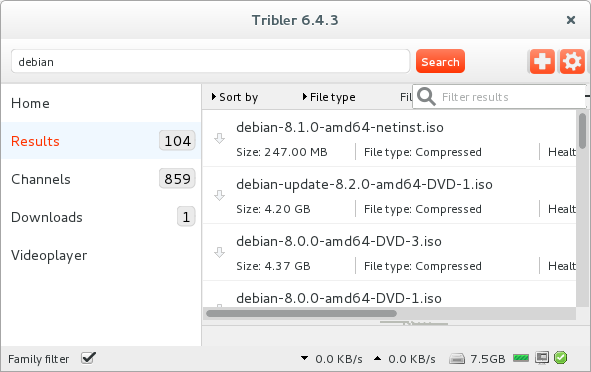
\includegraphics[scale=0.6]{introduction/figs/tribler-screenshot.png}}
%	\caption{Screenshot of Tribler v6.4.3.}
%	\label{fig:tribler-screenshot}
%\end{figure}

For years Tribler has received many contributions from students, staff and the open-source community.
This led to the degradation of structure and code quality of the Tribler code base.
Moreover, there has been done little profiling to detect bottlenecks in the code.
Finding and resolving bottlenecks in a complex code base such as Tribler's are often non-trivial yet an excellent way to increase responsiveness and performance.
For example, performing a blocking network request to a non or poorly responsive server can make the whole program grind to a halt, rendering the GUI non-responsive and leaving the user guessing what happened.
By making such a request non-blocking, the GUI remains responsive while the request is handled in the background.
In the meantime, changing such a request to become non-blocking goes well with refactoring the current structure and quality of the code to become a coherent, well-tested whole.\\

Another motivating example can be found in a recent addition to Tribler's code base.
Within Tribler anonymous connections have been recently implemented using onion routing~\cite{Plak-anonymous,ruigrok-anonymous,tanaskoski-anonymous}.
These anonymous connections are called anon-tunnels in Tribler.
This feature allows users to anonymously download files from other users in the network, safeguarding their privacy.
Every data packet has to be encrypted with multiple encryption layers and forwarded by a number of intermediate hops between the leecher and seeder~\cite{Plak-anonymous,tanaskoski-anonymous}, each decrypting one layer of encryption.
The total cost of bandwidth per file is increased, because it has to be forwarded by multiple nodes.
Because a node in the network may become part of an anon-tunnel, the workload increases per node.
The anon-tunnels have been profiled by [stokkink et al.] \todo{cite to stok et al.} and the results showed that the tunnels are now bound by CPU.
As handling packets involves encryption or decryption and message serialization, which are CPU intensive tasks, one wants to optimize this process.
The result should be higher achievable download rates and a more responsive program.


\section{Objective and research questions}
\label{chp1:sct:objectives-research-questions}
The objective of this thesis is to improve the connectability, performance and responsiveness of Tribler while improving its code base and stability. 
This is done by focussing on removing bottlenecks present.
These improvements will be applied by means of refactoring current code, which is largely undocumented, poorly tested and unnecessary complex.
In general, projects facing similar issues can adopt the practices applied when changes made to the Tribler code base.\\

The research presented in this thesis was carried out in cooperation with the Tribler team. 
The Tribler team consists of both staff members of the Technical University of Delft as well as Bachelor and Master students.
In total Tribler has been in development for over 10 years and the project has received contributions from more than 40 contributors.
Using the knowledge of senior developers still present, known problems of Tribler could be noted down immediately to which resulted in a set of diverse tasks to complete.
Based on the objectives of Tribler, this thesis aims to answer the main research question formulated below.\\

\textbf{Main Research Question:} How can we improve Tribler's performance, responsiveness and code base by means of refactoring?\\

To answer this main research question, we have defined three research questions below. Each of these research questions will be justified as why they contribute to the main research question.\\

\textbf{Research Question 1:} How can we identify bottlenecks in a complex system such as Tribler?\\

Software projects such as Tribler are often dependent on libraries i.e. third party code and combine several components or modules to form a program.
To improve the performance of such a system, one needs to be able to identify bottlenecks.
Bottlenecks are parts of the code where often performance and responsiveness can be gained.
Sometimes by implementing a more efficient algorithm or by introducing parallelization these bottlenecks can be resolved.
Identifying these bottlenecks is the first step to resolve them.\\

\textbf{Research Question 2:} Can a system such as Tribler benefit from asynchronous programming?\\

To improve performance and responsiveness, parts of Tribler can be rewritten to become asynchronous.
By performing tasks asynchronously the performance and responsiveness of a program can improve. 
An example of such a scenario was given in the previous section.
However, an asynchronous approach can have its drawbacks. 
One of these drawbacks is that it requires a different mindset for the programmers as the whole call chain and structure of a program becomes different.
Identifying these drawbacks and deciding if the benefits outweigh the costs is necessary to prevent the current state from worsening. \\

\noindent
\textbf{Research Question 3:} How can a complex code base such as Tribler's be effectively refactored to reduce complexity while improving performance?\\

By refactoring complex code, we strive to make Tribler's code base less complex and easier for new contributors to get familiar with.
This reduces effort required to start contributing to Tribler which hopefully acts as a motivating factor.
Identifying complex structures and means to refactor them in such a way that it reduces the complexity is therefore needed.

\section{Main contributions}
The main contribution this thesis offers are as follows. We present methods to identify bottlenecks in a complex system such as Tribler. 
Identifying bottlenecks is the first step of improving a system. While this thesis focuses on Tribler, similar approaches for different projects are possible.
Next, we provide arguments where asynchronous programming is preferred over synchronous programming in the context of the python programming language, using Tribler as a case study.
Finally, experimental results and measurements will be provided to confirm the main goal of this thesis i.e. improving responsiveness, code quality or performance have been achieved.

\section{Outline}
In this chapter we provided an introduction of this thesis and presented the research questions this thesis aims to answer. 
This section describes the other chapters in this thesis and their relevance to the research questions provided in section \ref{chp1:sct:objectives-research-questions}.
Chapter \ref{chp:preliminaries} provides preliminaries and terminology used through this thesis.
Chapter \ref{chp:problem-description} presents an overview of some of the problems Tribler is currently facing which this thesis addresses.
Chapter 
\todo{Add more here as cahpters are added.}
